\documentclass{article}
\usepackage[utf8]{inputenc}
\usepackage{siunitx}
\usepackage{graphics}
\usepackage[american,siunitx]{circuitikz}
\usepackage{amsmath}
\usepackage{svg} 
\usepackage{booktabs}
\usepackage{float}
\usepackage{xparse, xfp}
\usepackage{graphicx} 
\usepackage{steinmetz}
\usepackage{multirow}
\usepackage{pdfpages}
%\renewcommand{\thesubsection}{\thesection.\alph{subsection}}
\newcommand{\equal}{=}
\newcommand*\circled[1]{\tikz[baseline=(char.base)]{
    \node[shape=circle,draw,inner sep=1pt] (char) {#1};}}

\title{ECE 2101L\\Electrical Circuit Analysis II Laboratory\\\,\\Lab 7\\Input and Output Impedances of AC Black Boxes\\\,\\Report\\}
\author{Choi Tim Antony Yung}

\begin{document}

\clearpage\maketitle
\thispagestyle{empty}

\newpage
\setcounter{page}{1}

\section*{Objective}
The purpose of this experiment is to study the method of determining input and output impedances of AC black boxes from measurements.

\section{Measuring input impedance of a black box}
\begin{center}
    \begin{circuitikz}
        \draw
        (0,0) node[circ,label=180:\circled{1}]{} 
            to[sinusoidal voltage source, l_=$5\phase{0^{\circ}}$] (0,-2) 
            node[ground,label=180:0]{}
        (0,0) to[short,i=I] ++(1,0) 
            to[R,l_=$R_0\equal\SI{130}{\ohm}$] ++(2,0) -- ++(0.5,0) 
            node[circ,label={[label distance=-0.1cm]135:\circled{2}}]{} -- ++(0.5,0)
            to[R,l=$R_1\equal\SI{51}{\ohm}$] ++(2,0)
            node[circ,label={45:\circled{3}}](3){}
            to[R,l_=$R_2\equal\SI{620}{\ohm}$] ++(0,-2)
        (3) -- ++(1,0) to[C,l=$C\equal\SI{33}{\micro\farad}$] ++(0,-2) -- (0,-2)
        ;
        \draw [dashed] (3.5,1) -- ++(0,-3.5) -- ++(6,0) -- ++(0,3.5) -- ++(-6,0);
    \end{circuitikz}
\end{center}

\begin{figure}[h]
    \centering
        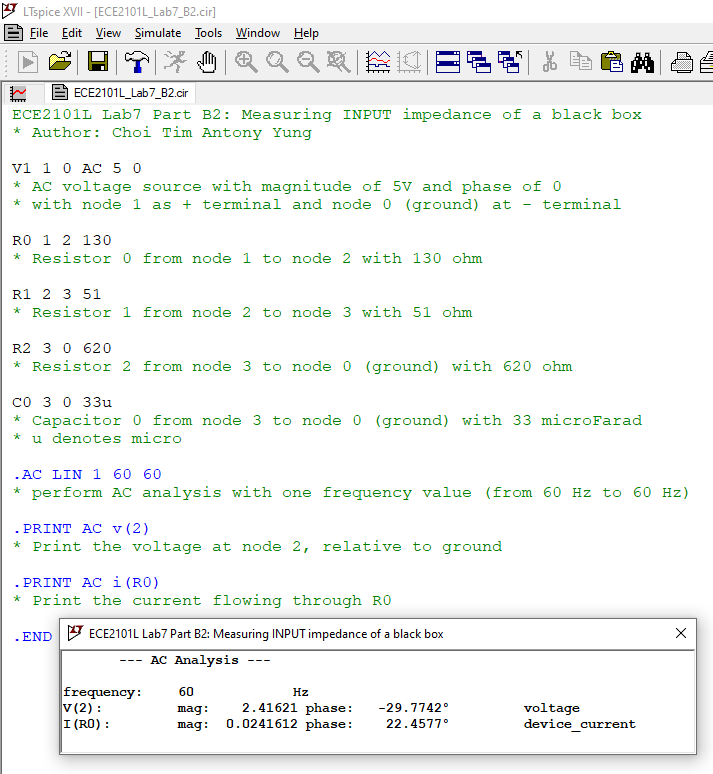
\includegraphics[scale=0.5]{sim_B2.png}
        \caption{Screenshot of circuit description used and the simulation result}
\end{figure}
\subsection*{Procedure}
A SPICE netlist was written to simulate the above circuit with LTspice XVI, the netlist is attached at the back of this report. The current of $R_0$ was used to determine $I$.

\subsection*{Result}
\begin{table}[H]
    \centering
    \resizebox{\columnwidth}{!}{%
    \begin{tabular}{rrr}
        \toprule
        $V_2$&$I$&$Z_{in}$\\
        calculated&calculated&calculated\\
        \midrule
        2.41621\phase{-29.7742^{\circ}}\,V&0.0241612\phase{22.4577^{\circ}}\,A&100.0037\phase{-52.2319^{\circ}}\,$\Omega$\\
        \bottomrule
    \end{tabular} 
    }
\end{table}
\begin{table}[H]
    \centering
    \resizebox{\columnwidth}{!}{%
    \begin{tabular}{rrrrrrr}
        \toprule
        $V_2$&$I$&$Z_{in}$&$|Z_{in}|$ Error\\
        measured&measured&measured&\\
        \midrule
        2.41621\phase{-29.7742^{\circ}}\,V&0.0241612\phase{22.4577^{\circ}}\,A&100.0037\phase{-52.2319^{\circ}}\,$\Omega$&0\,\%\\
        \bottomrule
    \end{tabular} 
    }
\end{table}
\subsection*{Analysis}
As the above measurement was simulated, there is no error. However, were it to be measured from an actual circuit, the measurement would be subjected to errors due to variation of impedance from its nominal value, imprecise oscilloscope measurement, dissipation of energy from nonideal wire, and noise from electromagnetic interferences, to name a few. Possible improvements to the above problem includes measuring impedances with LCR meter and adjusting impedance by adding small impedances, avoiding long wires, and spacing apart components, et cetera.

\newpage

\section{Measuring output impedance of a black box}
\begin{center}
    \begin{circuitikz}
        \draw
        (0,0) 
            node[circ,label=above:\circled{1}]{} 
            to[sinusoidal voltage source, l_=$6\phase{0^{\circ}}$] (0,-3) 
        (0,0) 
            to[R,l=$R_a\equal\SI{43}{\ohm}$] ++(3,0) 
            node[circ,label={[label distance=1]above:\circled{2}}](2){}
            to[C,l=$C_2\equal\SI{1000}{\micro\farad}$] ++(3,0)
            node[circ,label={above:\circled{3}}](3){}
            -- ++(0,-0.25) to[R,l_=$R_b\equal\SI{51}{\ohm}$] ++(0,-1.5)
            node[circ,label={[label distance=1]left:\circled{4}}]{}
            to[C,l_=$C_3\equal\SI{20}{\pico\farad}$] ++(0,-1) -- ++(0,-0.25) 
        (2) to[C,l_=$C_1\equal\SI{10}{\pico\farad}$] ++(0,-3)
        (3) to[C,l=$C_4\equal\SI{470}{\micro\farad}$] ++(2,0) -- ++(1.5,0) 
            node[circ,label=right:A]{}
            to[R,v=$v_0(t)$,l=$R$] ++(0,-3)  
            node[circ,label=right:B]{} -- (0,-3)
        ;
        \draw [dashed] (-1.5,1) -- ++(0,-4.5) -- ++(9.5,0) -- ++(0,4.5) -- ++(-9.5,0);
    \end{circuitikz}
\end{center}

\subsection*{Theory}

With $V_{th}$ as the open circuit voltage difference of A and B, and $V_{01}$ and $V_{02}$ as the voltage of $R=\SI{130}{\ohm}$ and $R=\SI{130}{\ohm}$ respectively, the magnitude of output impedance $R_{out}$ and $X_{out}$ can be found by solving the following system of equations:

$$|V_{01}|=\frac{R_1}{\sqrt{(R_1+R_{out})^2+(X_{out})^2}}|V_{th}|$$
$$|V_{02}|=\frac{R_2}{\sqrt{(R_2+R_{out})^2+(X_{out})^2}}|V_{th}|$$\\

... which can be simplified to the following:
$$(R_1+R_{out})^2+(X_{out})^2=\left(\frac{R_1}{|V_{01}|}|V_{th}|\right)^2$$
$$(R_2+R_{out})^2+(X_{out})^2=\left(\frac{R_2}{|V_{02}|}|V_{th}|\right)^2$$

By solving the above system of equation above, we can determine the magnitude of $R_{out}$ and $X_{out}$.

\subsection*{Procedure}
A SPICE netlist was written for the blackbox subcircuit, and three separate netlists was written to simulate, in LTspice XVI, the above circuit with A to B open or with different value of resistance attached to A and B, the netlists are attached at the back of this report. 

\begin{figure}[H]
    \centering
        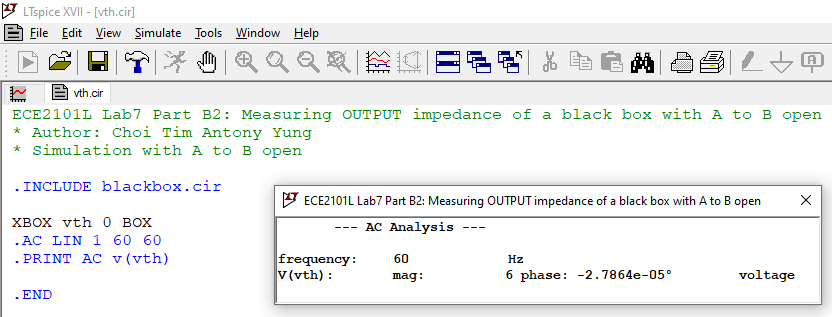
\includegraphics[scale=0.5]{sim_vth.png}
        \caption{Screenshot of circuit description used and the simulation result leaving A and B open}
\end{figure}

\begin{figure}[H]
    \centering
        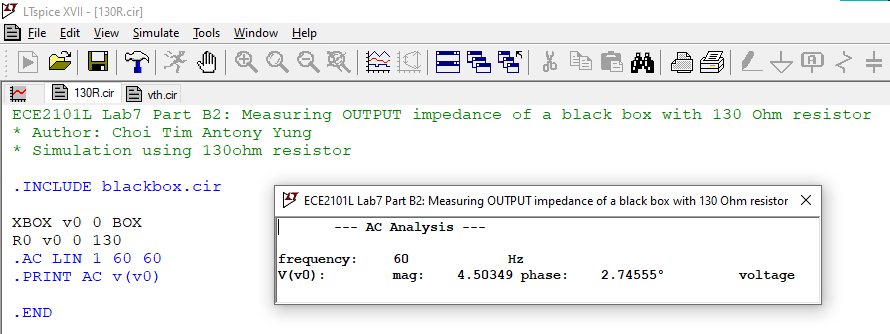
\includegraphics[scale=0.5]{sim_v0_130.png}
        \caption{Screenshot of circuit description used and the simulation result with \SI{130}{\ohm} resistor attached}
\end{figure}

\begin{figure}[H]
    \centering
        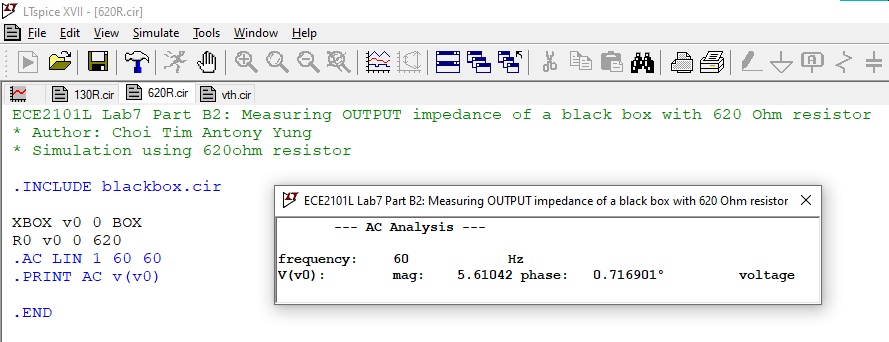
\includegraphics[scale=0.5]{sim_v0_620.png}
        \caption{Screenshot of circuit description used and the simulation result with \SI{620}{\ohm} resistor attached}
\end{figure}

\subsection*{Result}
\begin{table}[H]
    \centering
    \resizebox{\columnwidth}{!}{%
    \begin{tabular}{rrrrrrrr}
        \toprule
        R&$|V_{th}|$&$|V_0|$&$|R_{out}|$&$|X_{out}|$\\
        &measured&measured&calculated&calculated\\
        \midrule
        \SI{130}{\ohm}&\SI{6}{\volt}&\SI{4.50349}{\volt}&\multirow{2}{*}{\SI{43}{\ohm}}&\multirow{2}{*}{\SI{8.3}{\ohm}}\\
        \SI{620}{\ohm}&\SI{6}{\volt}&\SI{5.61042}{\volt}&&\\
        \bottomrule
    \end{tabular} }
\end{table}

\subsection*{Analysis}
After obtaining the value of the output impedance, we can repeat the measurement with an inductor L attached in series before R. In theory, if $X_{out}$ is inductive and therefore positive, then adding L in series will increase the magnitude of total reactance. Whereas if $X_{out}$ is capacitive therefore negative, then adding L, a positive reactance, in series will decrease the magnitude of total reactance. Therefore, if the measurement of $|X_{out}|$ after adding L is larger than before, then $X_{out}$ is inductive and therefore positive, otherwise, it is capacitive and therefore negative.

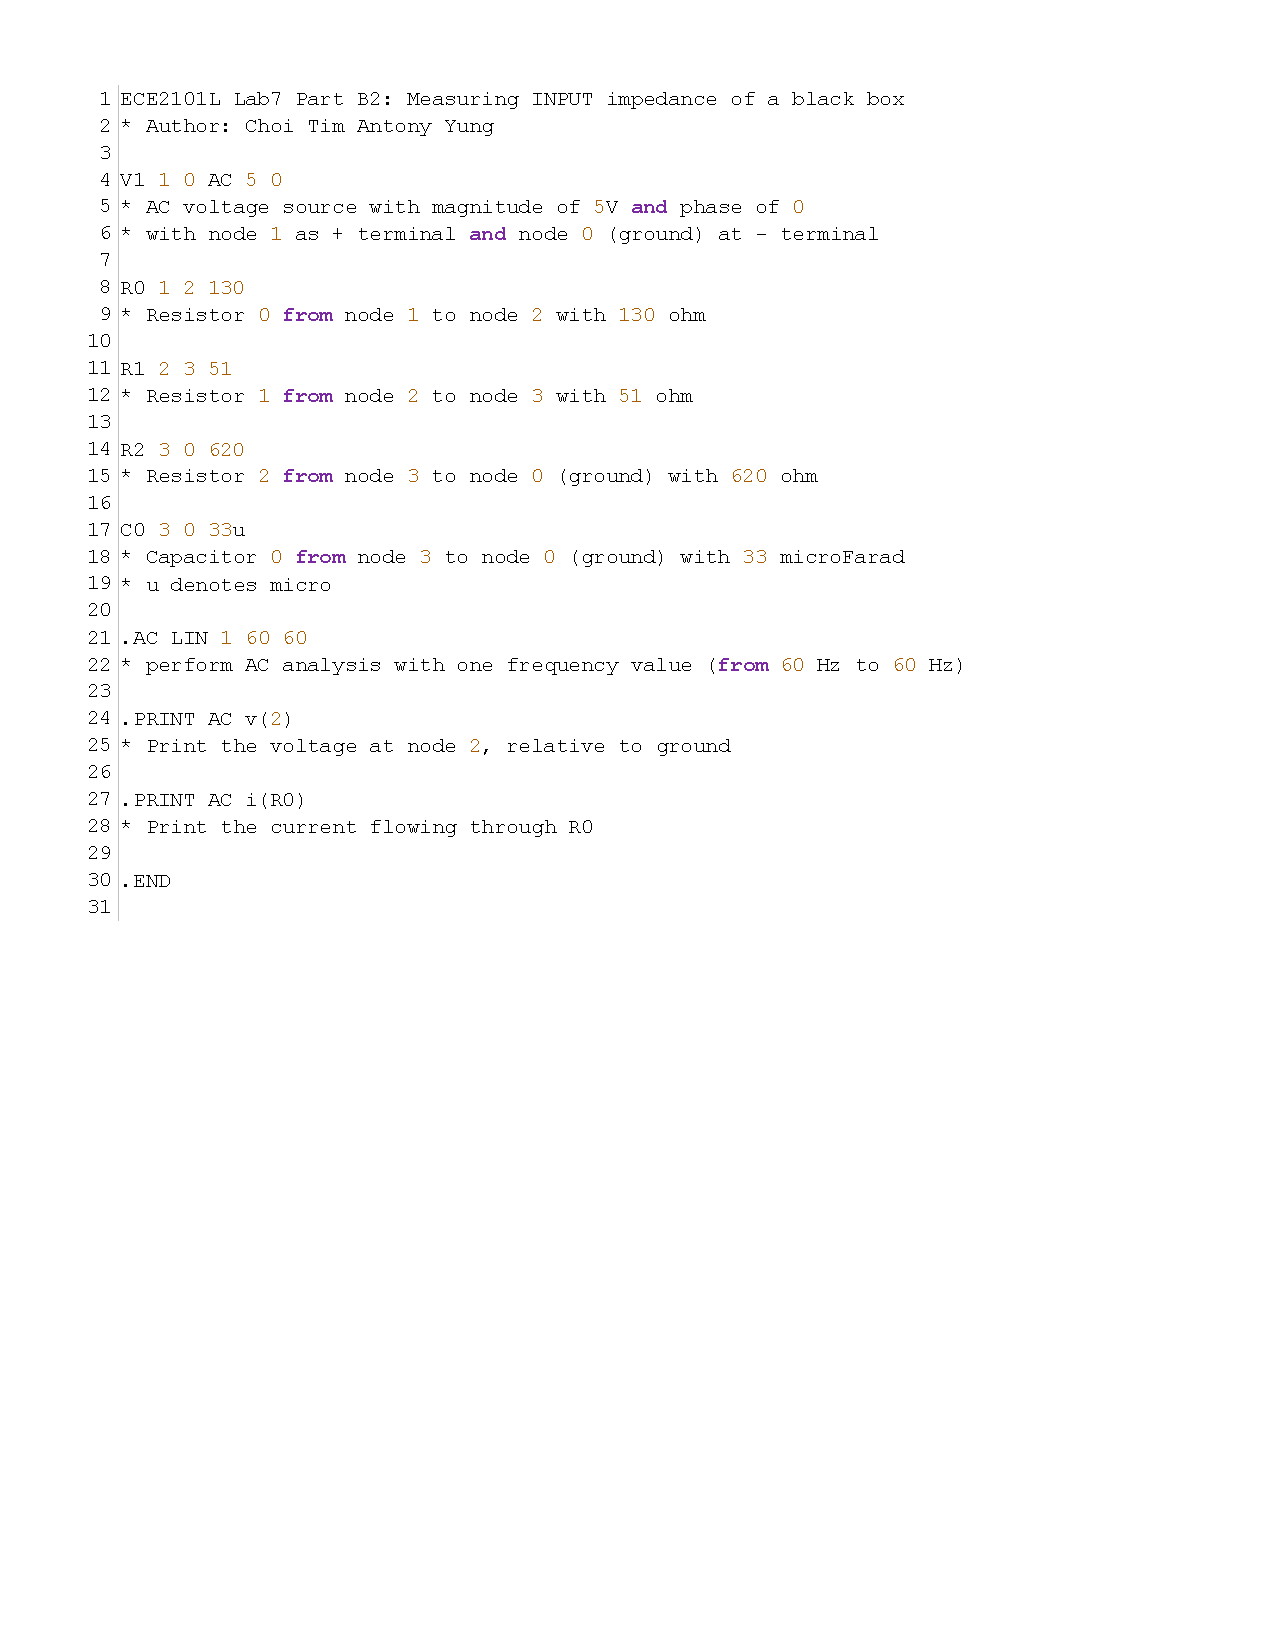
\includepdf[page={1}]{B2.cir.pdf}
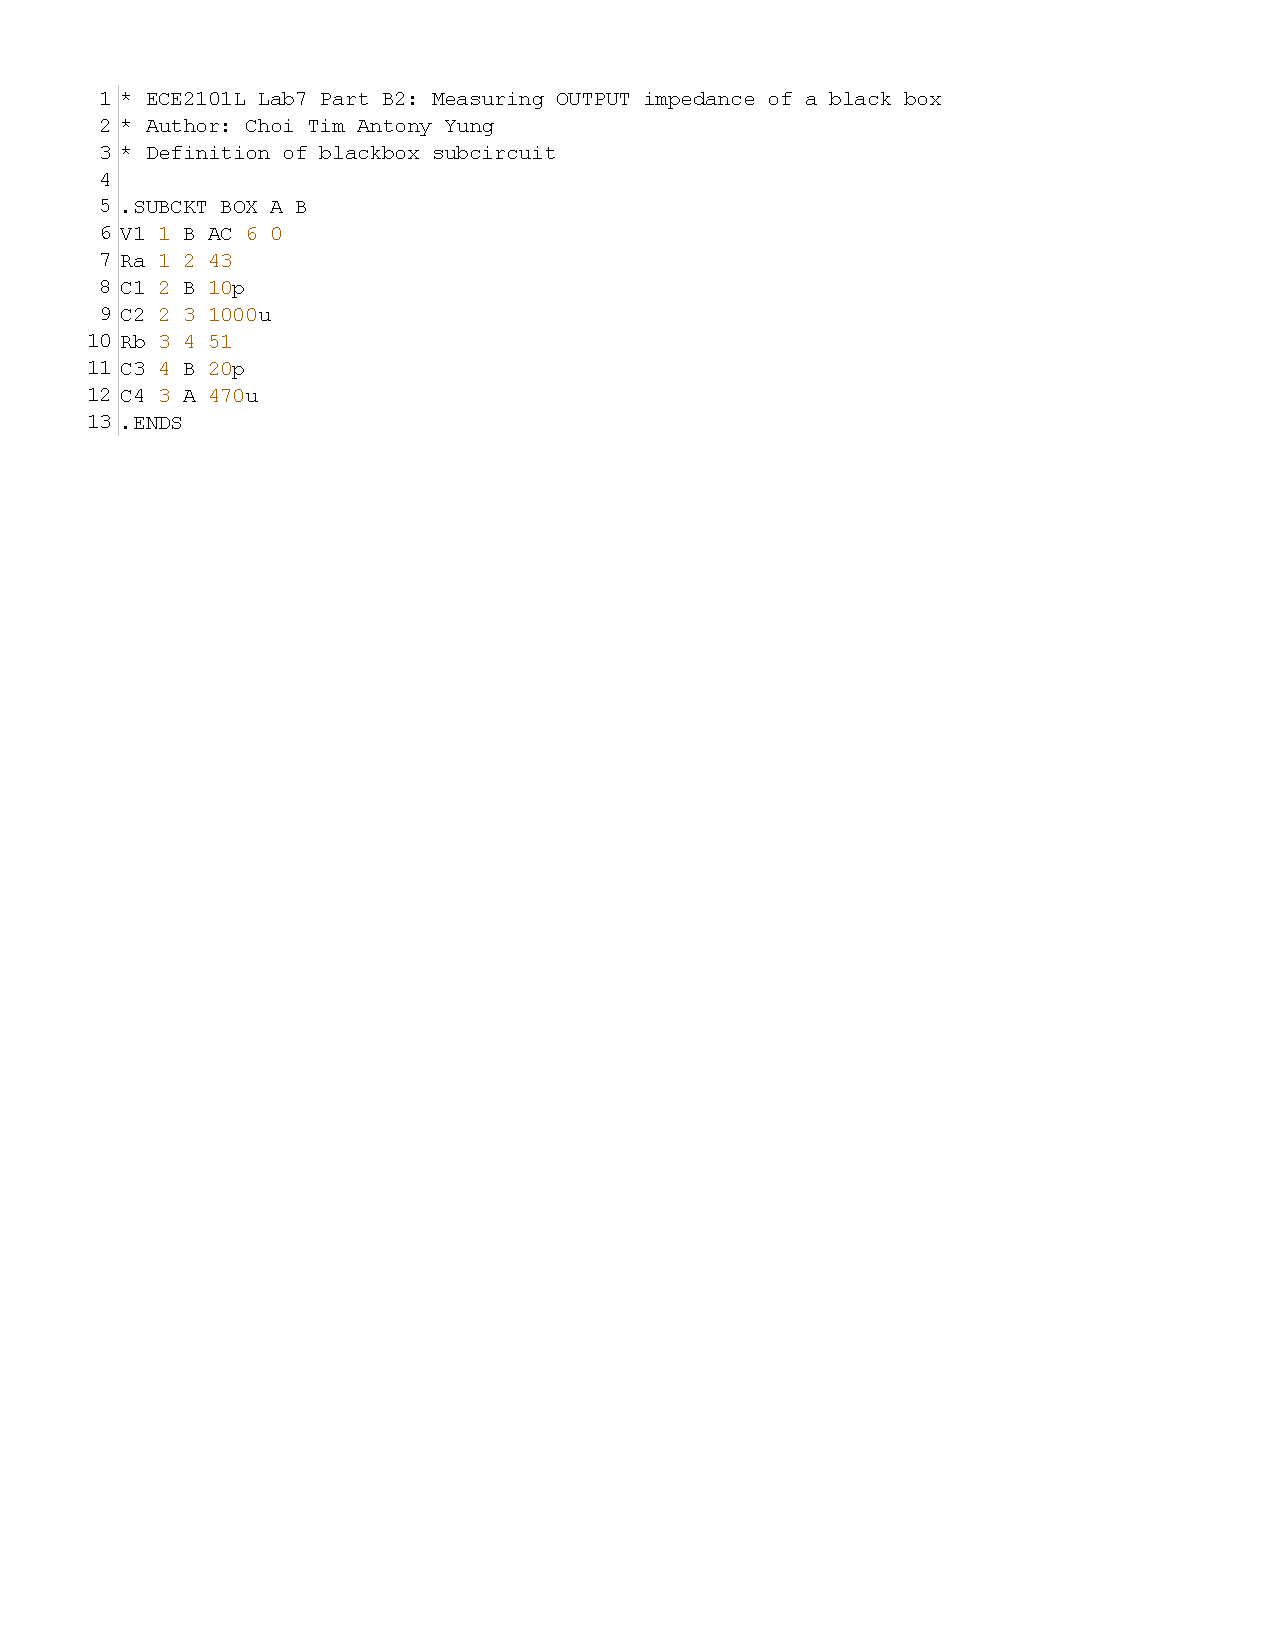
\includepdf[page={1}]{blackbox.cir.pdf}
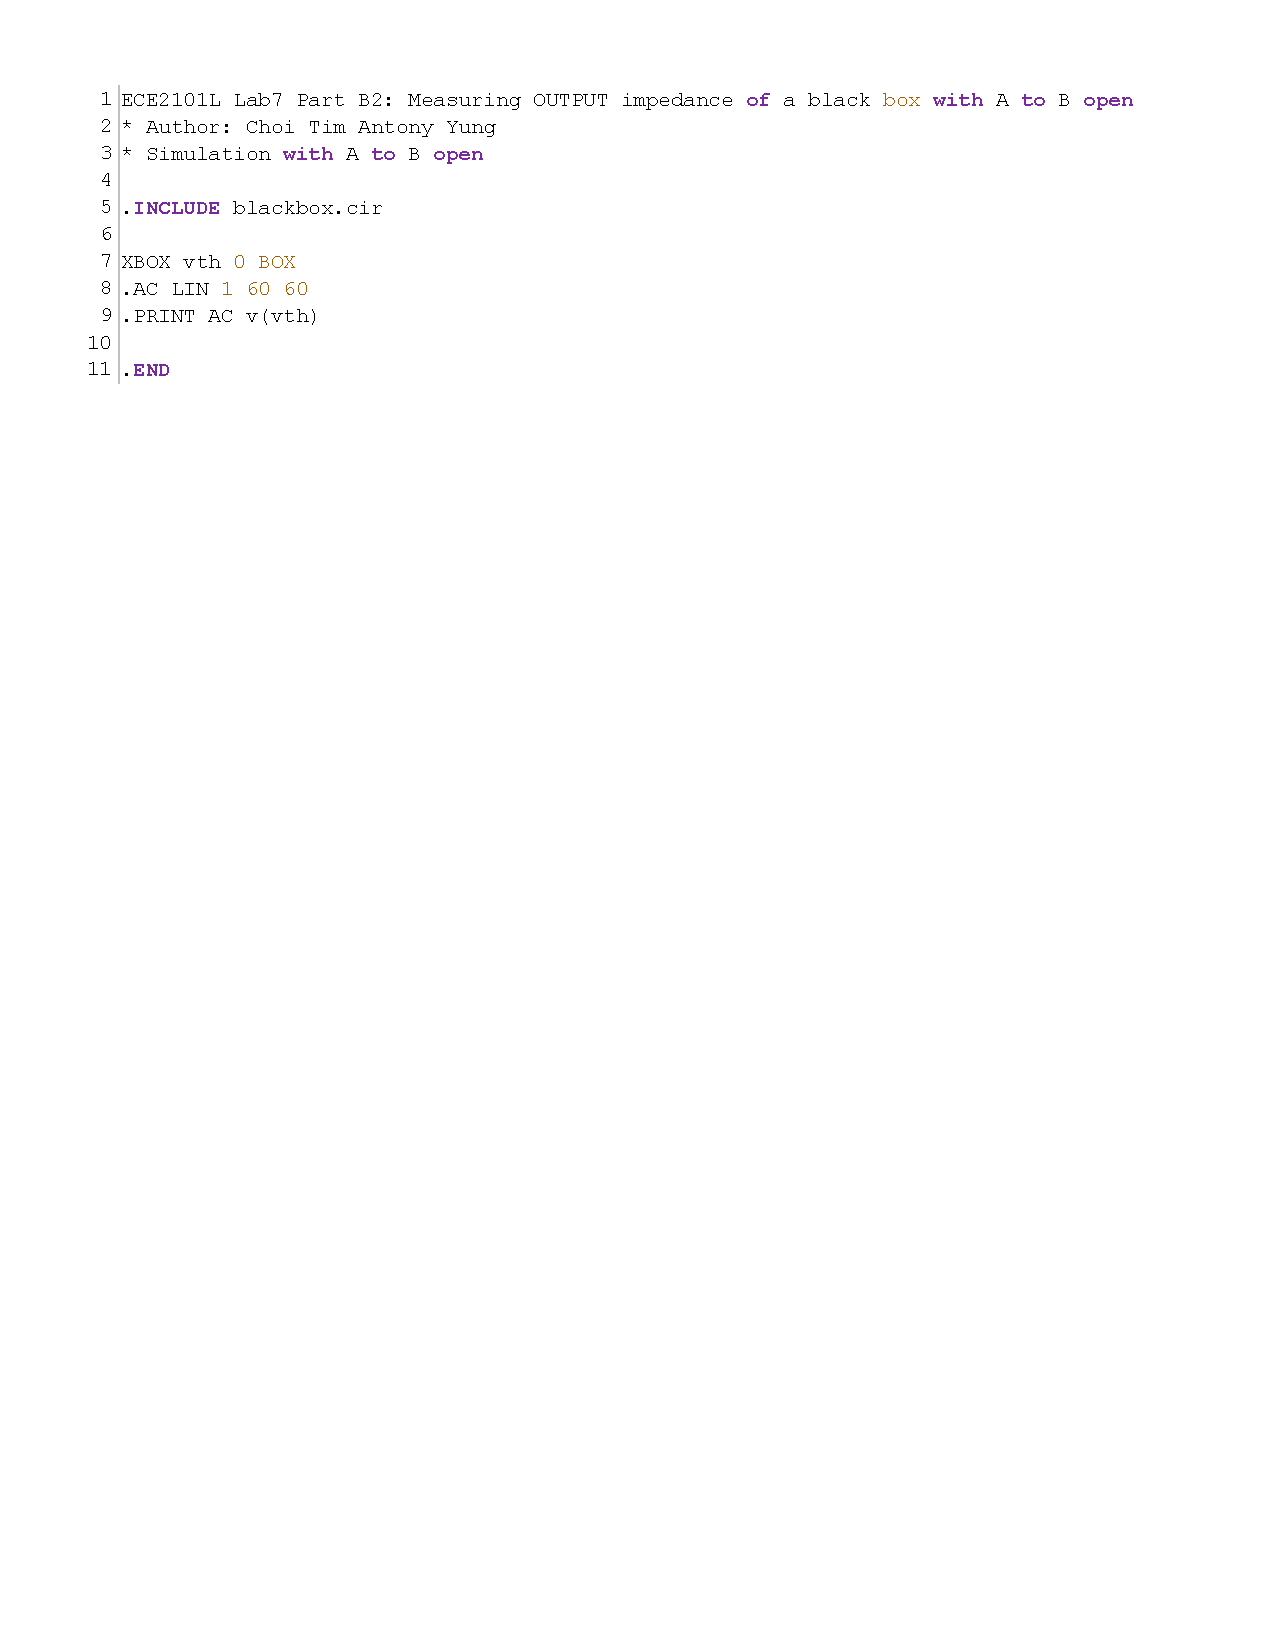
\includepdf[page={1}]{vth.cir.pdf}
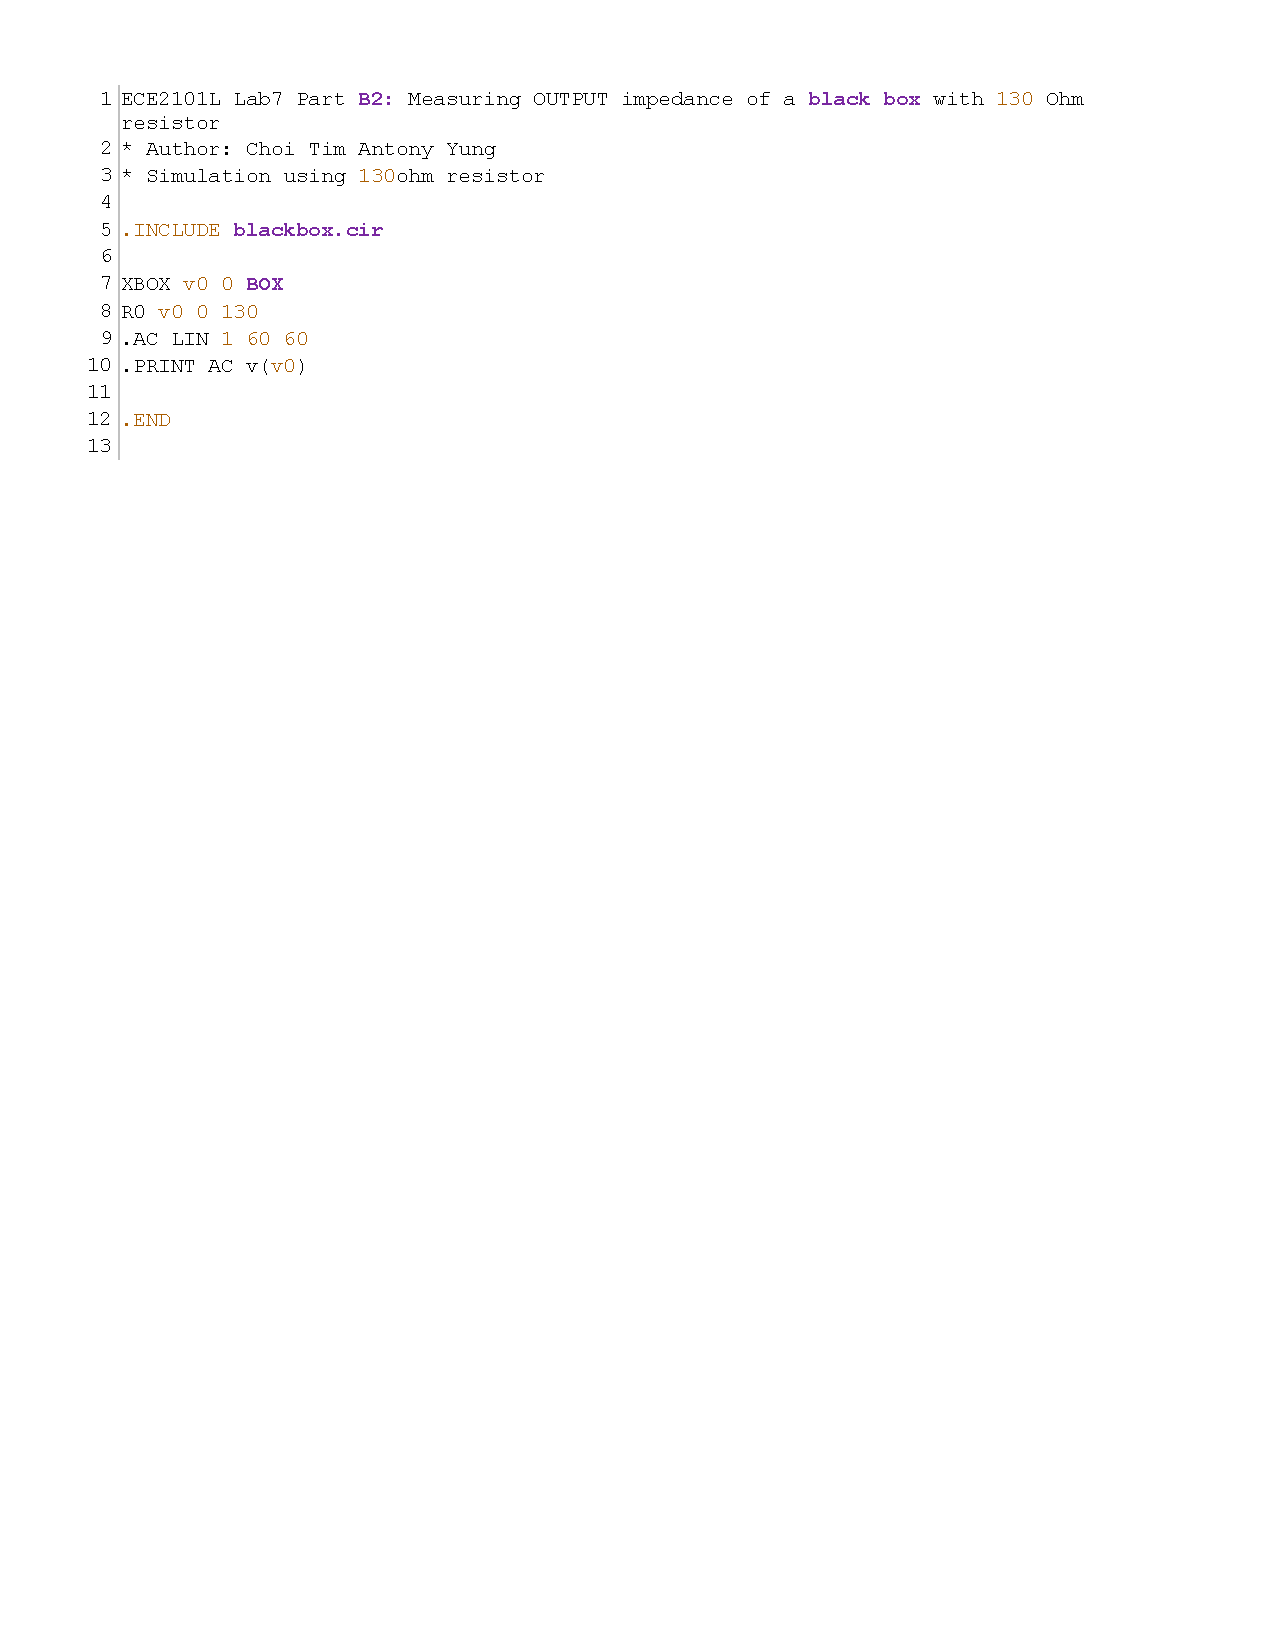
\includepdf[page={1}]{v01.cir.pdf}
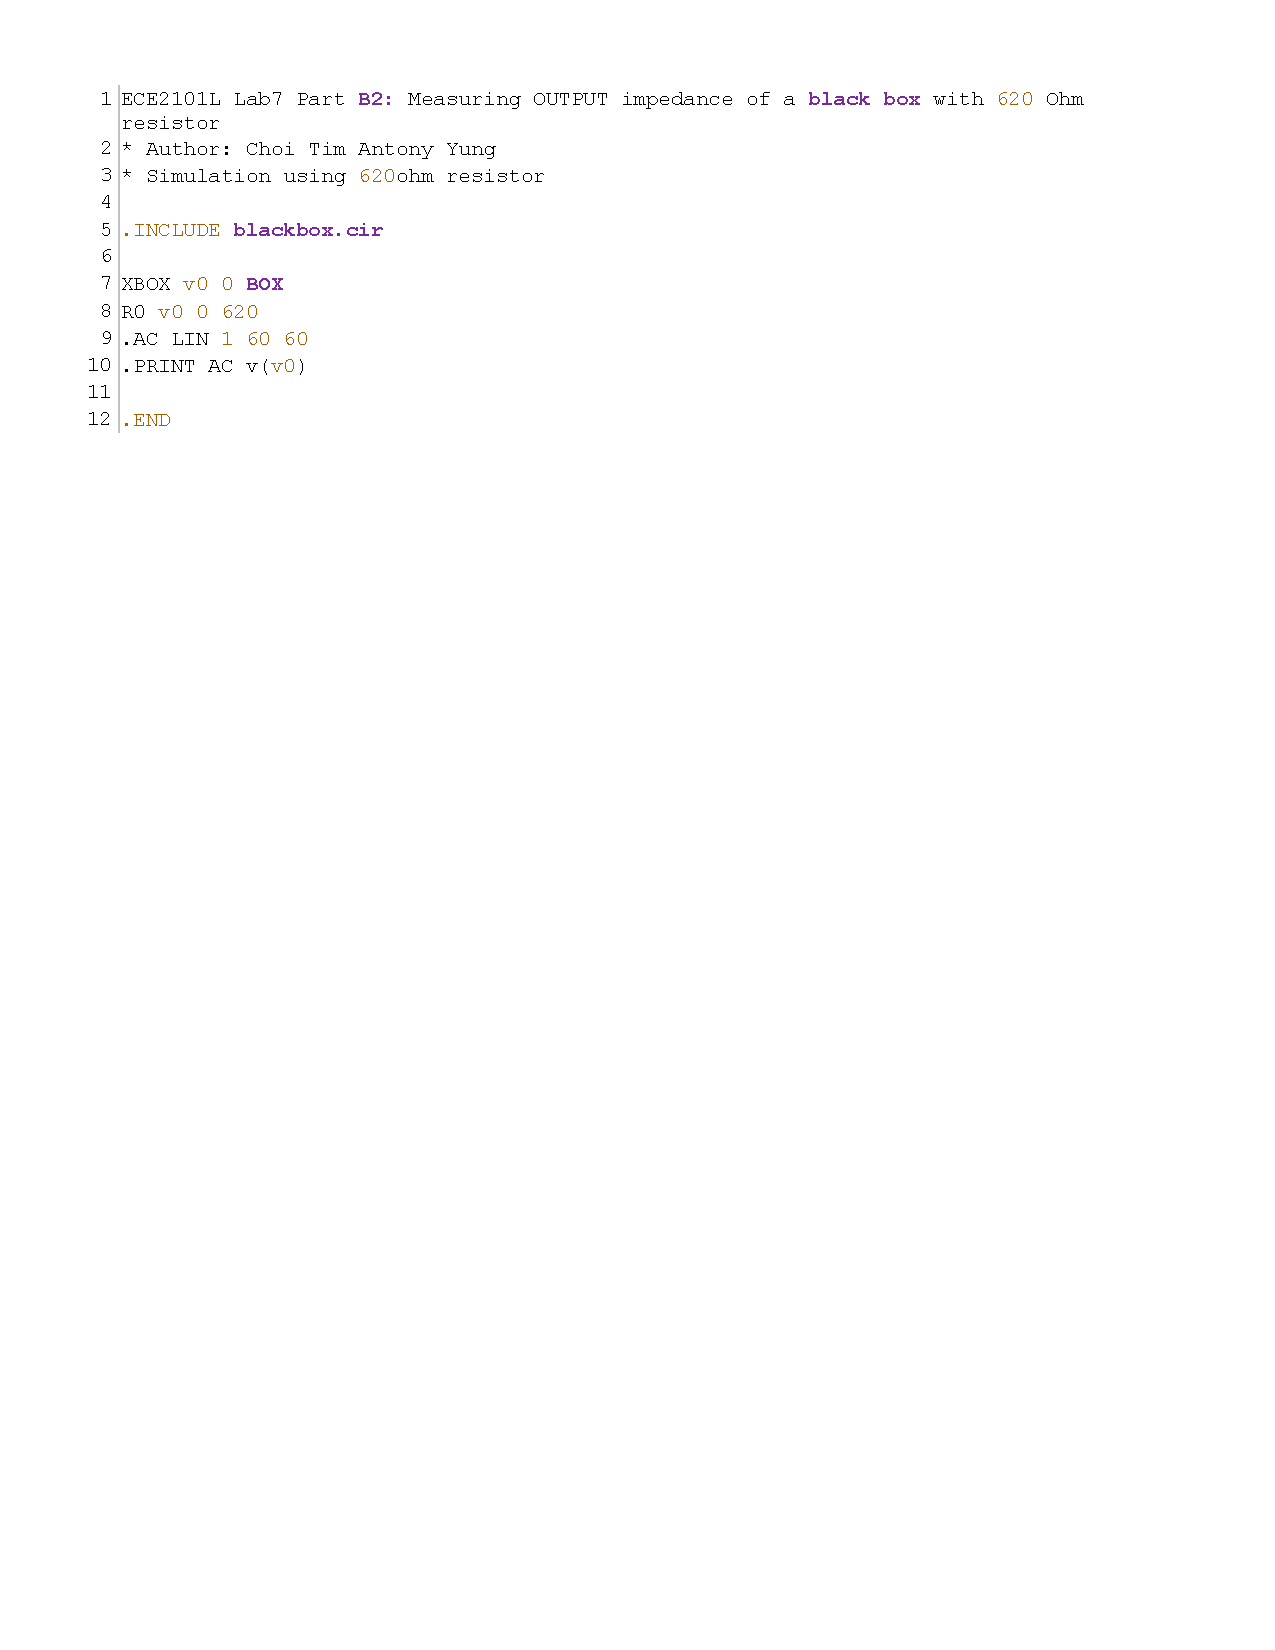
\includepdf[page={1}]{v02.cir.pdf}

\end{document}

